\definecolor{ttqqff}{rgb}{0.33,0.33,0.33}
%dash pattern=on 5pt off 2pt
%[fill = white, rounded corners = 4pt, inner sep = 1pt]
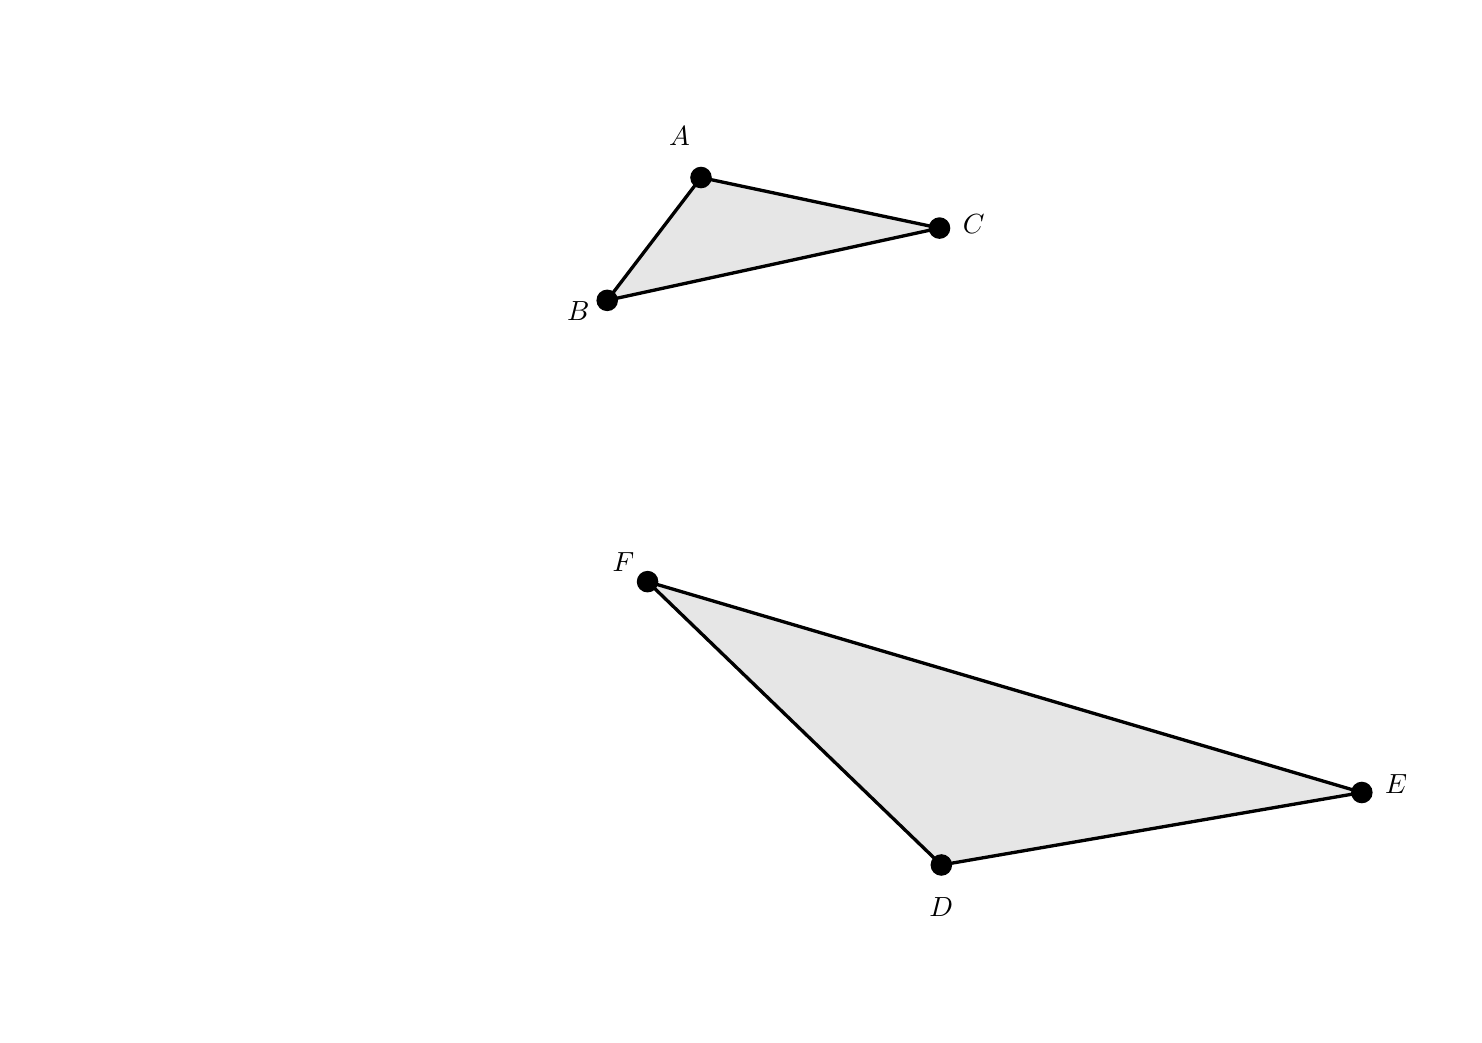
\begin{tikzpicture}[scale = 0.26]
    \clip(-26.68,-15.89) rectangle (42.99,32.35);
    \fill[line width=0pt,color=ttqqff,fill=ttqqff,fill opacity=0.15] (6.21,25.03) -- (1.63,19.03) -- (17.86,22.56) -- cycle;
    \fill[line width=0pt,color=ttqqff,fill=ttqqff,fill opacity=0.15] (17.95,-8.55) -- (38.49,-5.01) -- (3.6,5.29) -- cycle;
    \draw [line width=1.2pt] (6.21,25.03)-- (1.63,19.03);
    \draw [line width=1.2pt] (1.63,19.03)-- (17.86,22.56);
    \draw [line width=1.2pt] (17.86,22.56)-- (6.21,25.03);
    \draw [line width=1.2pt] (17.95,-8.55)-- (38.49,-5.01);
    \draw [line width=1.2pt] (38.49,-5.01)-- (3.6,5.29);
    \draw [line width=1.2pt] (3.6,5.29)-- (17.95,-8.55);
    \begin{scriptsize}
        \normalsize
        \fill [color=black] (1.63,19.03) circle (15pt);
        \draw[color=black] (0.22,18.5) node {$B$};
        \fill [color=black] (17.86,22.56) circle (15pt);
        \draw[color=black] (19.53,22.74) node {$C$};
        \fill [color=black] (6.21,25.03) circle (15pt);
        \draw[color=black] (5.16,27.06) node {$A$};
        \fill [color=black] (17.95,-8.55) circle (15pt);
        \draw[color=black] (17.94,-10.6) node {$D$};
        \fill [color=black] (38.49,-5.01) circle (15pt);
        \draw[color=black] (40.17,-4.6) node {$E$};
        \fill [color=black] (3.6,5.29) circle (15pt);
        \draw[color=black] (2.42,6.24) node {$F$};
    \end{scriptsize}
\end{tikzpicture}